A conversational intake is the first structured exchange between the author and the book machine. Its purpose is to turn a loose writing idea into a machine-readable project brief that can drive outline generation, section planning, and later editorial work. Rather than asking for a finished manuscript, the system asks a small bank of targeted questions that establish the book's identity, scope, and production constraints.

The intake begins with the title. The title is not merely a label; it is the anchor for the work object, the repository layout, and the eventual compiled artifact. From there, the system asks for the purpose of the book: what the author wants the book to explain, demonstrate, or accomplish. Purpose gives the outline its direction and helps distinguish a technical paper, a tutorial, a design memo, or a reflective essay.

The next questions identify the intended audience and the reader takeaway. Audience describes who the book is for, including their likely background and expectations. Reader takeaway states what a reader should understand, be able to do, or be persuaded of after finishing the book. These two fields are complementary: audience constrains the level of explanation, while takeaway clarifies the outcome the manuscript should produce.

The intake also captures voice and genre. Voice describes the authorial stance the system should preserve, such as formal, explanatory, experimental, or conversational. Genre identifies the kind of document being produced, such as a technical paper, proposal, handbook, or narrative report. Together, voice and genre shape the tone of the generated outline and the style of the section drafts that follow.

A separate design specification question records how the manuscript should be presented. This may include structural preferences, formatting expectations, diagram density, citation style, or other production constraints that affect the shape of the final artifact. The design spec is important because the book machine does not treat prose as isolated text; it treats prose as one coordinated artifact among outlines, references, diagrams, logs, and compiled outputs.

Finally, the intake asks about artifact structure. This question establishes how the work should be organized into chapters, sections, appendices, or other units, and it gives the system an initial sense of the manuscript's granularity. In practice, artifact structure becomes the scaffold for the canonical work object, the section payloads, and the repository files that hold the evolving draft.

Taken together, the question bank converts author intent into a durable starting state. It does not attempt to solve the whole writing problem at once. Instead, it captures the minimum information needed to normalize the project into a structured outline, so that later agents can draft sections, register references, request diagrams, and maintain coherence across the manuscript.

Figure~\ref{fig:ch03_sec01_conversation_intake} summarizes the intake as a linked sequence of questions that moves from identity to purpose, from purpose to audience and takeaway, and from there to voice, genre, design constraints, and artifact structure. That progression matters because it mirrors the way the system stabilizes a project: first by naming it, then by clarifying what it is for, and finally by constraining how it should be written and assembled.

\begin{figure}[htbp]
\centering
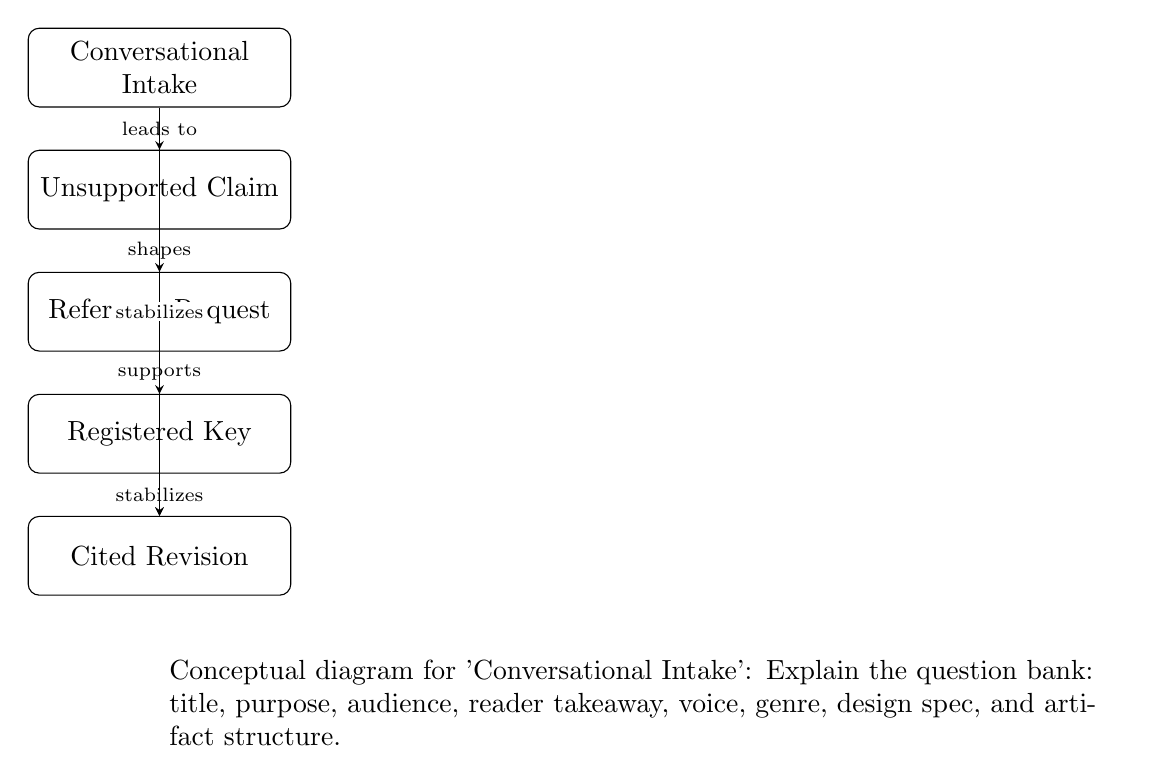
\begin{tikzpicture}[>=stealth, node distance=2.2cm,
  concept/.style={draw, rounded corners, align=center, text width=3.1cm, minimum height=1cm},
  relation/.style={font=\scriptsize, fill=white, inner sep=1pt}]
\node[concept] (n1) at (0,0.0) {Conversational Intake};
\node[concept] (n2) at (0,-1.55) {Unsupported Claim};
\node[concept] (n3) at (0,-3.1) {Reference Request};
\node[concept] (n4) at (0,-4.65) {Registered Key};
\node[concept] (n5) at (0,-6.2) {Cited Revision};
\draw[->] (n1) -- node[relation] {leads to} (n2);
\draw[->] (n2) -- node[relation] {shapes} (n3);
\draw[->] (n3) -- node[relation] {supports} (n4);
\draw[->] (n4) -- node[relation] {stabilizes} (n5);
\draw[->] (n1) -- node[relation] {stabilizes} (n5);
\node[align=left, text width=12cm, anchor=north west] at (0,-7.4) {Conceptual diagram for 'Conversational Intake': Explain the question bank: title, purpose, audience, reader takeaway, voice, genre, design spec, and artifact structure.};
\end{tikzpicture}

\caption{Conceptual diagram for Conversational Intake: the question bank captures title, purpose, audience, reader takeaway, voice, genre, design spec, and artifact structure.}
\label{fig:ch03_sec01_conversation_intake}
\end{figure}
